\chapter{Introduction} % Write in your own chapter title
\label{Chapter1}
\lhead{Chapter 1. \emph{Introduction}} % Write in your own chapter title to set the page header

\section{Introduction}

In recent years, surveillance cameras are becoming very popular and placed almost everywhere, e.g. stations, airports, banks, shops, streets. It is hard to keep a balance between security and privacy. A person may feel protected when he knows himself and his surroundings are being observed. But at the same time he may feel uncomfortable because he does not know how many cameras are set and from what angle they are pointing at him.

The information that a person probably wants to know most about the cameras is their viewing fields, e.g. whether he is being observed. It is almost impossible to find cameras without any support in real scene. There is a generally known technology which can be applied for purposes like this: Mixed Reality (MR). MR is the encompassing of both Augmented Reality and Augmented Virtuality, merging real world in which we are living and virtual worlds created by computers. It produces new environments where real and virtual entities can co-exist and interact in realtime. Mixed Reality applications are usually equipped with Head Mounted Display (HMD) as shown in figure \ref{fig:HMD}.

\begin{figure}[htbp]
  \centering
    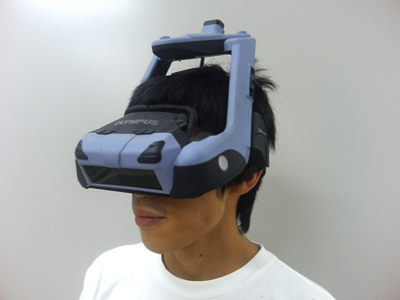
\includegraphics{./Primitives/hmd.jpg}
    \rule{35em}{0.5pt}
  \caption[An HMD]{An HMD}
  \label{fig:HMD}
\end{figure}

However, HMDs are bulky and inconvenient for outdoor applications, as discussed in \citep{Reference2} \citep{Reference4}. In place of that, mobile devices like the one in figure \ref{fig:VAIO}, equipped with built-in camera, Global Positioning System (GPS) and gyrocompass devices, have been found practical and are a topic of many researches \citep{Reference2} \citep{Reference4}. Such devices find their high potential use in outdoor MR applications and researches because of their small size, high specifications, and competitive prices compared to normal laptops.

\begin{figure}[htbp]
  \centering
    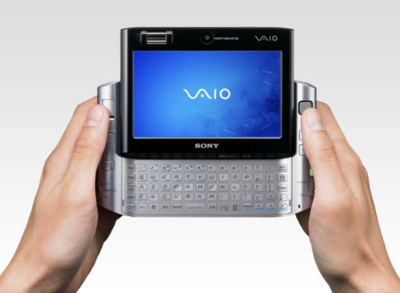
\includegraphics{./Primitives/vaio.png}
    \rule{35em}{0.5pt}
  \caption[A SONY VAIO mobile device]{A SONY VAIO mobile device}
  \label{fig:VAIO}
\end{figure}

In this research, we propose a combination of such mobile devices and outdoor MR to enable a user to easily have a visualization of viewing fields of surveillance cameras surrounding him. The main part of this research is to find the best methods to visualize the viewing fields of the surveillance cameras.

\section{A use case}

In order to get visualized images of the viewing fields of surrounding surveillance cameras in a certain direction, the typical usage scenario is:

\begin{enumerate}
\item The user points the mobile camera in that direction and takes video of the scene.
\item The mobile device is equipped with a camera, GPS and gyrocompass devices. The camera lets the user take video from his own point of view. GPS and gyrocompass devices give the system the position and orientation of the mobile camera, respectively.
\item The video is processed to integrate the visualization about the viewing field of the surrounding surveillance cameras.
\item The integrated video is rendered on the screen of the mobile device so that the user can see.
\end{enumerate}

An example is shown in Figure [cite, cite, cite]:
\begin{itemize}
\item Figure [cite] shows the position of the user, the mobile device, and the a surveillance camera in the world coordinates.
\item The user is taking video using the camera on the mobile device, at the position and in the direction as shown in Figure [cite].
\item The original video taken by the camera is shown in Figure [cite]. This video is not rendered on the screen.
\item The viewing field of the surveillance camera is visualized on the original video, then this video is rendered on the screen as shown in Figure [cite].
\item When the user changes the position or orientation of the mobile camera, the video and the visualized viewing field of the surveillance camera will also change accordingly.
\end{itemize}

The above example only demonstrates one kind of visualization method, which may not be the best one, only to show how the system works. Five visualization methods are proposed in this research and are described in chapter \ref{Chapter3}.
